\documentclass[tikz,border=3pt]{standalone}
\usepackage[T1]{fontenc}
\usepackage{times}
\usepackage{xcolor}
\usepackage{tikz}
\usepackage{pgfplots}
\pgfplotsset{compat=1.18}

\definecolor{huntrixblue}{HTML}{1F5A7A}
\definecolor{huntrixteal}{HTML}{2A8C82}

\begin{document}
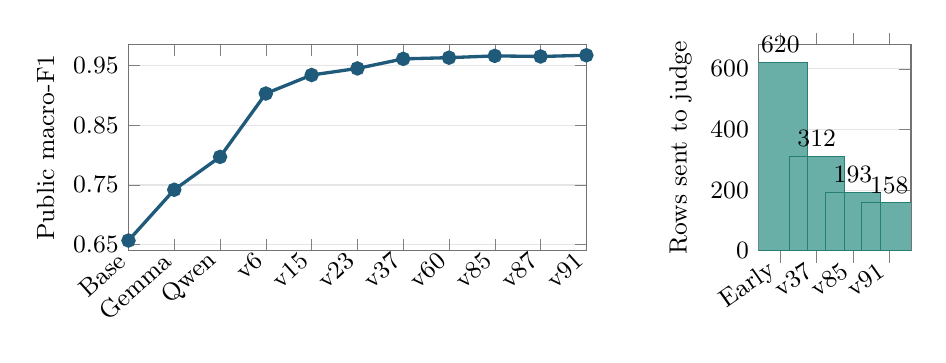
\begin{tikzpicture}
\begin{axis}[
  at={(0,0)}, anchor=west,
  width=0.61\textwidth, height=42mm,
  xmin=0, xmax=10, ymin=0.64, ymax=0.985,
  xtick={0,1,2,3,4,5,6,7,8,9,10},
  xticklabels={Base,Gemma,Qwen,v6,v15,v23,v37,v60,v85,v87,v91},
  x tick label style={font=\small,rotate=42,anchor=east},
  ytick={0.65,0.75,0.85,0.95}, tick label style={font=\small},
  ylabel={Public macro-F1}, label style={font=\small},
  ymajorgrids, grid style={black!10}, axis line style={draw=black!55}
]
\addplot[huntrixblue, very thick, mark=*, mark size=2pt]
coordinates {(0,0.657) (1,0.742) (2,0.797) (3,0.903) (4,0.934)
 (5,0.945) (6,0.961) (7,0.963) (8,0.966) (9,0.965) (10,0.967)};
\end{axis}
\begin{axis}[
  at={(0.66\textwidth,0)}, anchor=west,
  width=0.29\textwidth, height=42mm,
  ybar, bar width=7mm, ymin=0, ymax=680,
  ylabel={Rows sent to judge}, label style={font=\small},
  symbolic x coords={Early,v37,v85,v91}, xtick=data,
  x tick label style={font=\small,rotate=35,anchor=east},
  tick label style={font=\small}, nodes near coords,
  nodes near coords style={font=\small}, ymajorgrids,
  grid style={black!10}, axis line style={draw=black!55},
  enlarge x limits=0.2
]
\addplot[fill=huntrixteal!70, draw=huntrixteal!90!black]
coordinates {(Early,620) (v37,312) (v85,193) (v91,158)};
\end{axis}
\end{tikzpicture}
\end{document}
